\chapter{Introduction \& Summary}

%Provide a short summary of the whole PhD thesis:
% -Introduction to QC & CQED
% -Building Blocks of Superconducting Quantum Processors
% -Realization of a Two-Transmon QP
% -Tune-Up & Characterization of the Universal Two-Qubit Gate
% -Grover's Algorithm: Introduction & Background
% -Implementation on the Two-Qubit Processor
% -Design of a Scalable QC Architecture

\section{Quantum Computing \& Circuit Quantum Electrodynamics}

\begin{figure}
	\centering
		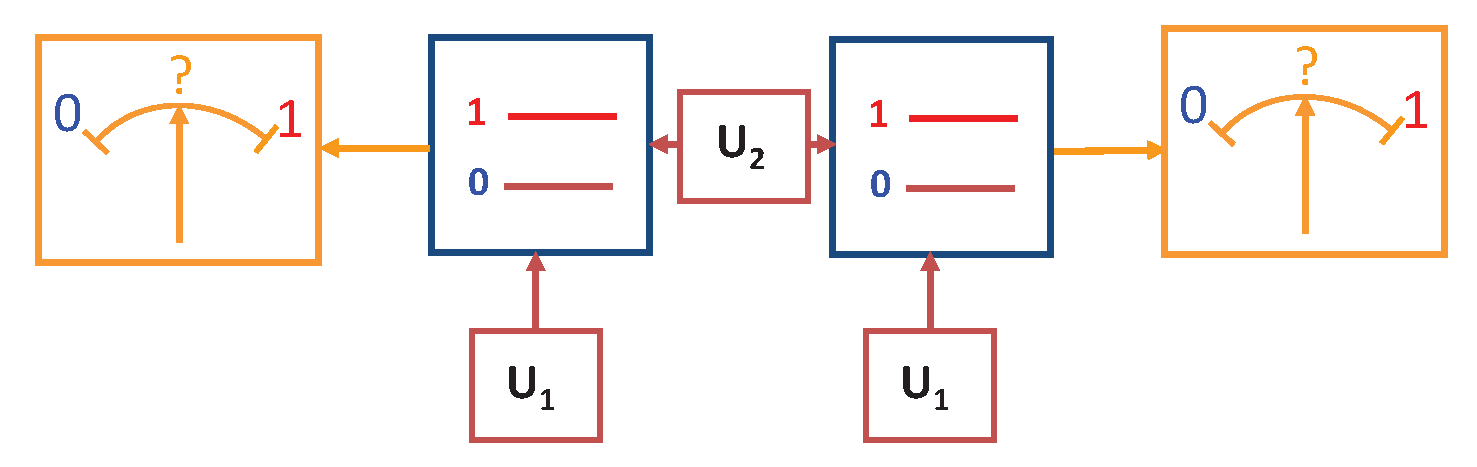
\includegraphics[width=0.8\textwidth]{./material/papers/grover/submission1/Fig1}
	\caption[Blueprint of a ``canonical'' two-qubit quantum processor]{The blueprint of a ``canonical'' two-qubit quantum processor. Shown are two qubits that can be individually manipulated ($U_1$) and are connected by a universal two-qubit gate $U_2$. Each of the qubits can be read out individually.}
	\label{fig:qubit_processor_blueprint}
\end{figure}

This thesis presents experiments performed with a superconducting two-qubit quantum processor. The main goal of this work was to demonstrate a possible quantum computing architecture based on superconducting qubits that follows the canonical blueprint of a quantum processor as shown in fig. \ref{fig:qubit_processor_blueprint}, in accordance with the five criteria formulated by \cite{divincenzo_physical_2000}. By this definition, a universal quantum computer is a register of well-defined quantum bits  (1) with long coherence times (2) on which one can perform universal single- and two-qubit quantum gates(3), read out the state of each qubit individually and with high fidelity (4) and reset the qubit register to a well-defined state (5).

Implementing this allegedly simple list of requirements in a system of superconducting qubits has been a major research challenge during the last decade. Incoherent quantum tunneling in a superconducting device was observed for the first time by \cite{devoret_measurements_1985,martinis_energy-level_1985} and \cite{clarke_quantum_1988}, which showed that it is possible to cool down a Josephson junction sufficiently to see quantum-mechanical tunneling between different quantum levels of the system. However, the observation of incoherent quantum tunneling did not prove that the quantum state of these devices could be manipulated coherently. The first demonstration of such coherent quantum behaviour in a superconducting system was achieved more than ten years later by \cite{nakamura_coherent_1999}, who measured for the first time coherent energy oscillations between two quantum levels of a Cooper pair box. This experiment created a large interest in superconducting quantum circuits and led to development of a research field on superconducting quantum computing. In the years after Nakamuras experiment, several types of superconducting qubits were proposed using Josephson junctions in different configurations to realize systems where e.g. the Josephson phase \citep{martinis_rabi_2002} or the magnetic flux inside a superconducting ring \citep{mooij_josephson_1999,chiorescu_coherent_2003} are the dominant quantum variables. In this context, an important result on the way to robust superconducting qubits was the development of the so-called {\it Quantronium} qubit by \cite{vion_manipulating_2002}. The Quantronium is a Cooper pair box with comparable Josephson and charging energies operated at a well-defined ``sweet spot'' at which the sensitivity of the device to charge and flux noise is greatly reduced. The high coherence times achieved with the Quantronium --values larger than 2 $\mu s$ have been reported-- allowed for the first time the implementation of NMR-like quantum operations using a superconducting qubit \citep{collin_nmr-like_2004}. Shortly after that, in 2004, the development of another new type of qubit, the so called {\it Transmon}, by \cite{wallraff_strong_2004} marked again a drastic improvement in coherence times, qubit robustness and usability. The Transmon qubit is a Cooper pair box shunted with a large capacitor that drastically decreases the charging energy of the system and thus renders the device almost insensitive to charge noise, however still leaving sufficient anharmonicity to operate the device as a qubit. With the Transmon, coherence times comparable or higher than those reported for the Quantronium have been achieved {\it without} operating the qubit at a special working point, thereby greatly reducing experimental complexity. Furthermore, by embedding the Transmon qubit in a superconducting coplanar waveguide (CPW) resonator it is possible to protect it from external sources of electrical noise and use the dispersive interaction between the qubit and the resonator for reading out the qubit state \citep{blais_cavity_2004}. This approach of embedding a superconducting qubit in a waveguide resonator has been termed --in analogy with conventional quantum electrodynamics-- {\it circuit quantum electrodyanmics} (CQED) and gained wide popularity in the superconducting qubit community \todo{add some citations of relevant experiments}. So far, using this CQED approach, superconducting quantum processors with up to three qubits have been realized and two- and three-qubit quantum gates \citep{fedorov_implementation_2011}, multi-qubit entanglement \citep{dicarlo_preparation_2010} and simple quantum algorithms \citep{dicarlo_demonstration_2009} as well as quantum error correction \citep{reed_realization_2011} have been demonstrated. Futhermore, experiments demonstrating fundamental quantum effects that before were accesible only in quantum optics have been performed, demonstrating e.g. QND measurements of photons in a cavity \citep{johnson_quantum_2010}, the resolution of photon-number states \citep{schuster_resolving_2007} and the measurement of the Autler-Townes and Mollow transitions with a superconducting qubit \citep{baur_measurement_2009}.

Recently, a new type of CQED architecture has been developed by \cite{paik_observation_2011} that combines Transmon qubits with 3D cavities instead of CPW resonators, resulting again in an impressive increase of qubit coherence times of up to two orders of magnitude, with reported qubit relaxation times as high as $80 \; \mu \mathrm{s}$\todo{verify this!} and decoherence times at a comparable time scale. These drastically improved coherence times have already made possible the realization of elemental quantum feedback and error correction schemes with these systems \todo{cite Irfan's paper here} and make them promising candidates for the realization of a superconducting quantum computer.\todo{expand this section as soon as new relevant material appears, include recent IBM, Yale}

In parallel to this, the development of quantum-limited amplifiers based on nonlinear superconducting resonators by \cite{siddiqi_rf-driven_2004} and \cite{vijay_invited_2009} provided a very useful tool for measuring and amplifying weak quantum signals, which was already used in several context within the field of superconducting qubits: By operating such a nonlinear amplifier in a hysteretic regime and coupling it, in analogy to the CQED approach, dispersively to a superconducting qubit, \cite{siddiqi_dispersive_2006} and \cite{mallet_single-shot_2009} were able to demonstrate a high-fidelity readout scheme for Transmon qubits, reaching up to 97 \% readout fidelity. \cite{vijay_observation_2011} used quantum-limited amplifiers to read out a Transmon qubit coupled to a linear microwave cavity and were able to observe quantum jumps of its state. \todo{Add Quantum Feedback Paper Here} used a similar setup with a 3D Transmon to implement a quantum feedback scheme to phase-stabilize a Rabi oscillation of a superconducting qubit.

\smallskip

With the research presented in this thesis we aim \comment{can I really say ``we'' here or should it be ``I''?} to complement the CQED architecture as outlined in the last sections by combining a multi-qubit architecture based on Transmon qubits with a readout scheme based on a nonlinear bifurcation amplifier, thus providing the so-far missing per-qubit single-shot readout that is needed to realize a canonical superconducting quantum processor with these devices.

The first part of the thesis discusses the realization of a superconducting two-qubit processor based on Transmon qubits fitted with individual single-shot readouts. With this processor, we implement elementary one- and two-qubit quantum operations and use it to run a simple quantum algorithm that demonstrates probabilistic quantum speed-up. Finally, we discuss the realization of a four-qubit quantum processor using a more scalable approach that could possibly be extended to an even larger number of qubits.

\section{Realizing a Two-Qubit Quantum Processor}

\begin{figure}[ht!]
	\centering
		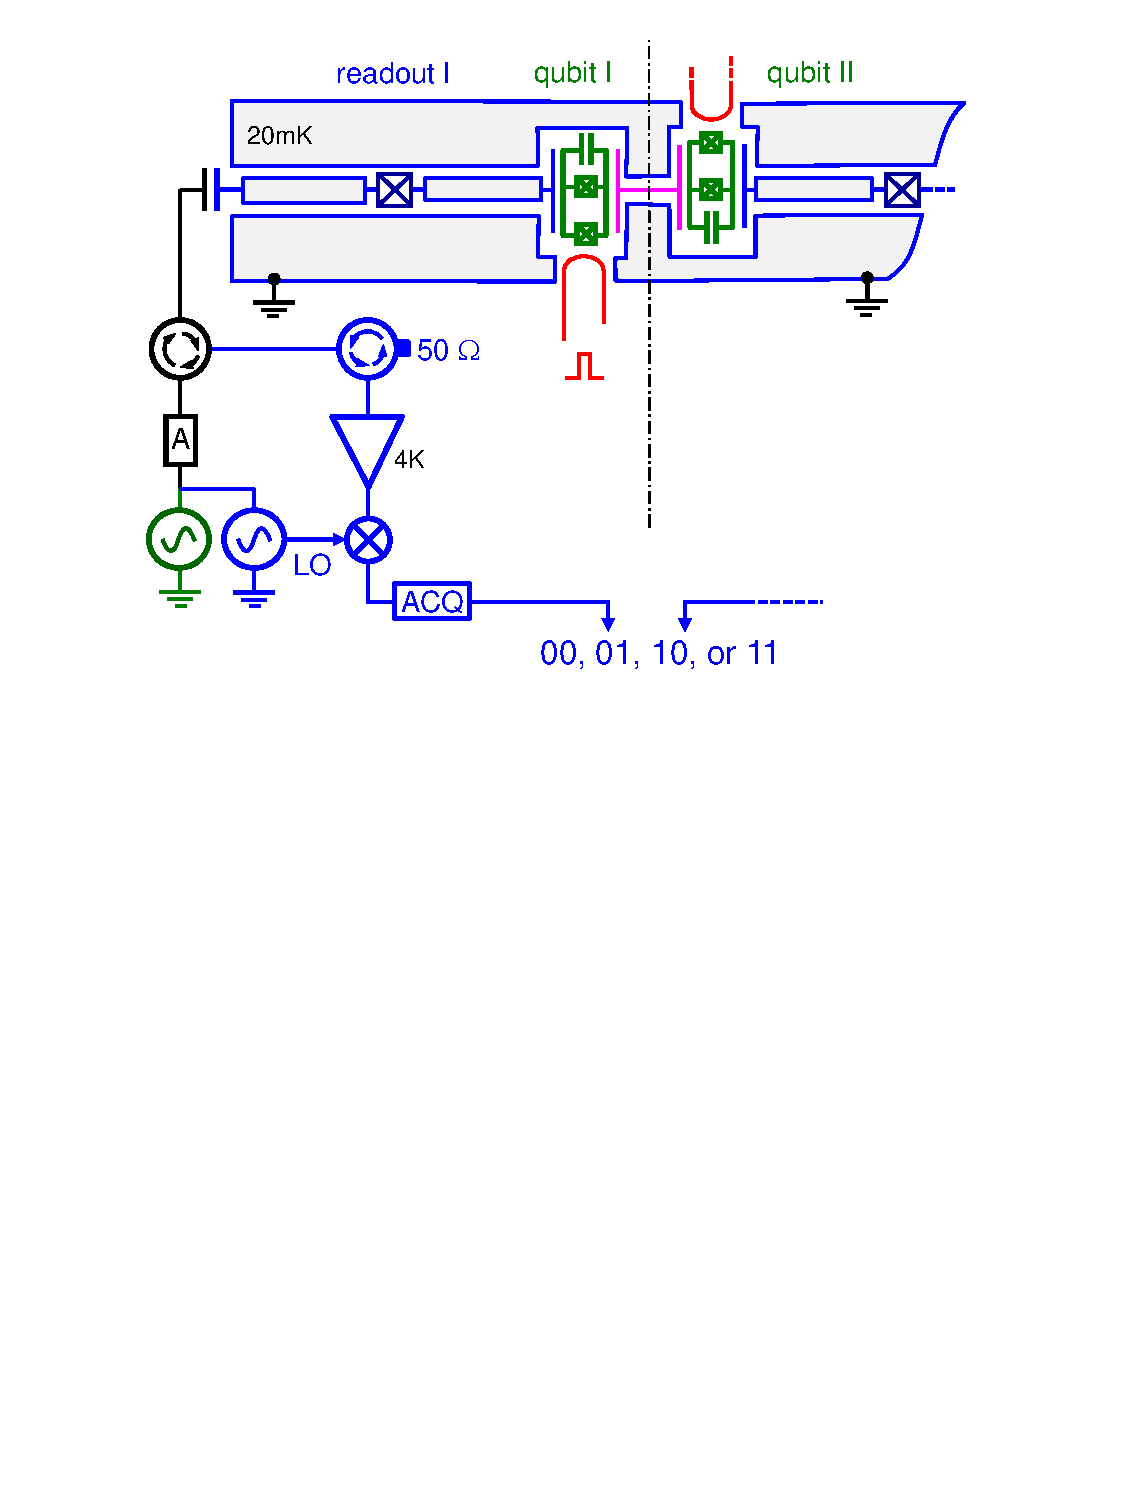
\includegraphics[width=0.75\textwidth]{./material/papers/grover/figures/2_qubit_processor_schematic}
	\caption[Circuit schematic of the realized two-qubit processor]{Circuit schematic of the two-qubit processor realized in this work, showing the two qubits in green, the qubit readouts in blue and the fast flux lines in red. Each qubit is embedded in its own nonlinear readout resonator and can be driven and read out through an individual microwave line.}
	\label{fig:two_qubit_processor_schematic}
\end{figure}

The quantum processor implemented in this work is shown in fig. \ref{fig:two_qubit_processor_schematic}. It consists of two superconducting quantum bits of the Transmon type, each equipped with its own drive and readout circuit. The qubit readout is realized using a nonlinear coplanar-waveguide resonator that serves as a so-called {\it cavity bifurcation amplifier} (CBA)\citep{siddiqi_dispersive_2006,mallet_single-shot_2009,vijay_invited_2009} and allows a single-shot readout of the qubit state. Each qubit can be manipulated by driving it with microwave pulses through its readout resonator, allowing for robust and fast single-qubit operations. The qubit frequencies can be tuned individually using fast flux lines, allowing us to change the frequency of each qubit over a range of several GHz. The coupling between the two qubits is realized through a fixed capacitance that connects the two top-electrodes of the Transmons and implements a fixed $\sigma_{xx}$-type qubit-qubit coupling. This coupling allows us to generate entangled two-qubit states and to implement a two-qubit gate. We use this simple processor to generate entangled two-qubit states, test the Bell inequality, implement an universal two-qubit gate and perform a simple quantum algorithm that demonstrates probabilistic quantum speed-up, as will be discussed in the following sections.

\section{Demonstrating Simultaneous Single-Shot Readout}

\begin{figure}[ht!]
	\centering
		\includegraphics[width=0.5\textwidth]{"./material/papers/grover/figures/s curves"}
\includegraphics[width=0.43\textwidth]{"./data/ct5/2011_04_21 - grover and tomo/good_data/readout only"}
	\caption[Switching probabilities of the two qubit readouts as a function of the readout excitation power]{a) Switching probabilities of the two qubit readouts as a function of the readout drive power at a fixed driving frequency. The measurement is performed after preparing the qubits in the states $\color{blue}{\ket{0}}$, $\color{red}{\ket{1}}$ and $\color{brown}{\ket{2}}$. The readout contrast is given as the difference in probability between the curves corresponding to the states $\color{blue}{\ket{0}}$ and $\color{red}{\ket{1}}$ or $\color{brown}{\ket{2}}$, respectively. The highest contrasts of 88 and 89 \% are achieved when the qubit is in state $\color{brown}{\ket{2}}$. b) Readout matrix of the two-qubit system. The matrix contains the probabilities of obtaining a given measurement result after having prepared the system in a given state. \figcomment{Replace this figure since it is not very intuitive. It would be better to show something which allows the reader to directly quantify the visibility and readout crosstalk present in the system.}}
	\label{fig:qubit_readout_characteristics}
\end{figure}

For the read out the qubit state we use a so called {\it cavity bifurcation amplifier} (CBA). This approach consists in capacitively coupling the qubit to a coplanar waveguide resonator that is rendered nonlinear by placing a Josephson junction in its center conductor. The capacitive coupling between the qubit and the resonator creates a dispersive interaction between them that induces a change of the resonance frequency of the resonator dependent on the state of the qubit, and vice versa. Furthermore, the resonator can exhibit bistability at certain drive parameters due to its nonlinearity. Therefore, by driving it at a carefully chosen frequency and drive amplitude we can use the dispersive qubit-resonator interaction to map the state of the qubit to one of the bistable states of the resonator. We can then stabilize this resonator state by changing its operating point, effectively freezing it from the further evolution of the qubit state. This allows us to measure the state of the resonator with high precision without being limited by qubit relaxation, thereby providing a high-fidelity, single-shot qubit readout. Contrary to other CQED approaches, in our setup each individual qubit is fitted with such a CBA readout, allowing hence a simultaneous readout of the full two-qubit register, following the canonical blueprint of a quantum computer as formulated by DiVincenzo. For single-qubit CBA readouts, readout fidelities up to 93 \% have been reported \citep{mallet_single-shot_2009}. However, due to the higher complexity and design contraints of our system, only  83-89 \% fidelity have been achieved for the processor presented here. The full characterization of the readout of our processor is shown in fig. \ref{fig:qubit_readout_characteristics}. Fig. \ref{fig:qubit_readout_characteristics}a shows the switching probabilities of each individual qubit readout as a function of the drive amplitude, measured at a fixed drive frequency. Individual curves correspond to the qubit being prepared in different states $\ket{0}$, $\ket{1}$ or $\ket{2}$, the difference between either two curves giving the readout contrast between those qubit states. Preparing the qubit in state $\ket{2}$ before readout can increase the readout fidelity by more than 10 \% and is therefore often used in the experiments presented in this thesis. Fig. \ref{fig:qubit_readout_characteristics}b shows the full readout matrix of the two-qubit register that relates measured readout switching probabilities with real qubit state occupation probabilities and allows us to correct readout errors when performing quantum state tomography. In the main text of this thesis we discuss all relevant readout fidelities and errors in details and analyze different error sources limiting the readout performance in our experiments.

\section{Generating and Characterizing Entanglement}

\begin{figure}
	\centering
		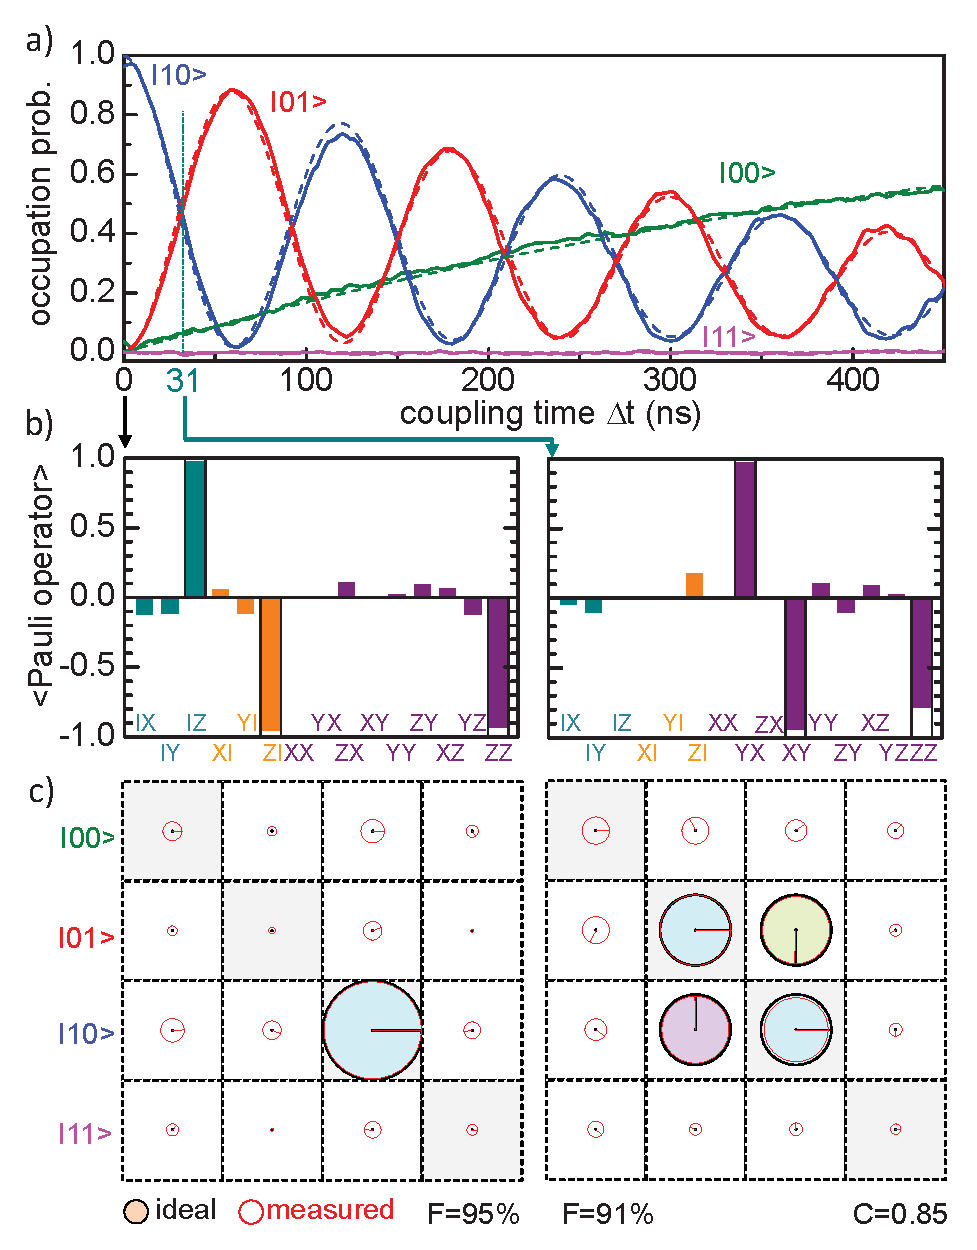
\includegraphics[width=0.7\textwidth]{./material/papers/iswap/submission1/Dewes_Figure2}
	\caption[Generating entangled two-qubit states by swapping interaction]{Energy oscillations between the two qubits induced by a resonant swapping interaction between them. a) The qubit state after switching on the swapping interaction for a given time $\Delta t$. The frequency of the oscillations corresponds to $2g = 8.7 \; \mathrm{MHz}$. b) The Pauli set of the two-qubit state measured at $0\; \mathrm{ns}$ and $31\; \mathrm{ns}$. c) The reconstructed density matrices corresponding to the two measured Pauli sets. In c), the area of each circle corresponds to the absolute value of each matrix element and the color and direction of the arrow give the phase of each element. The black circles correspond to the density matrices of the ideal states $\ket{10}$ and $1/\sqrt{2}/(\ket{10}+i\ket{01})$, respectively.\figcomment{verify sign!}}
	\label{fig:swap_interaction_state_tomography}
\end{figure}

The capacitive coupling between the two qubits provides a $\sigma_{xx}$-type interaction that can be used to generate entangled two-qubit states. Conveniently, this coupling is only effective when the qubit frequencies are near-resonant and can therefore be effectively switched on and off by tuning the qubit frequencies in and out of resonance. For the processor realized in this work, the effective coupling constant $g$ of the two qubits has been measured as $2g = 8.2 \; \mathrm{MHz}$. When the two qubits are in resonance, the effective Hamiltonian of the two-qubit system can be written as

\begin{equation}
	U(t)  =  \left( \begin{array}{cccc} 1 & 0 & 0 & 0 \\ 0 & \cos{2 \pi t g} & i\sin{2 \pi t g} & 0 \\ 0 & i\sin{2 \pi t g} & \cos{2 \pi t g} & 0 \\ 0 & 0 & 0 & 1 \end{array} \right) \label{eq:swap_evolution_operator}
\end{equation}
, where $U(t)$ is written in the basis $\{\ket{00},\ket{01},\ket{10},\ket{11}\}$. By using fast flux pulses to non-adiabatically tune the qubits in and out of resonance we can switch on this interaction for a well-defined time. We first characterize the effect of the coupling on the qubit register by preparing the state $\ket{10}$, tuning the qubits in resonance for a given time and measuring the  qubit state afterwards. The resulting curve is shown in fig. \ref{fig:swap_interaction_state_tomography} and clearly shows energy oscillations between the two qubits. Analyzing this curve allows us to extract the effective coupling strength between the qubits. Leaving the interaction between the qubits on for a well-defined time allows us to generate entangled Bell states that we characterize by performing quantum state tomography. The experimental reconstruction of the density matrix of such a Bell-state of the type $\ket{\psi} = 1/\sqrt{2}(\ket{01}+i\ket{10})$ is shown in fig. \ref{fig:swap_interaction_state_tomography}b. The measured fidelity of the prepared state of 91 \% and the concurrence of 85 \% confirm that entanglement is present in the system. We also characterize the entanglement between the two qubits by measuring the so-called {\it Clauser-Horne-Shimony-Holt} operator \citep{clauser_proposed_1969}, which combines measurements of the state of the two qubits along different axes on the Bloch sphere and provides a test that can distinguish between classical correlation and quantum entanglement in a two-qubit system.

\begin{figure}[ht!]
	\centering
		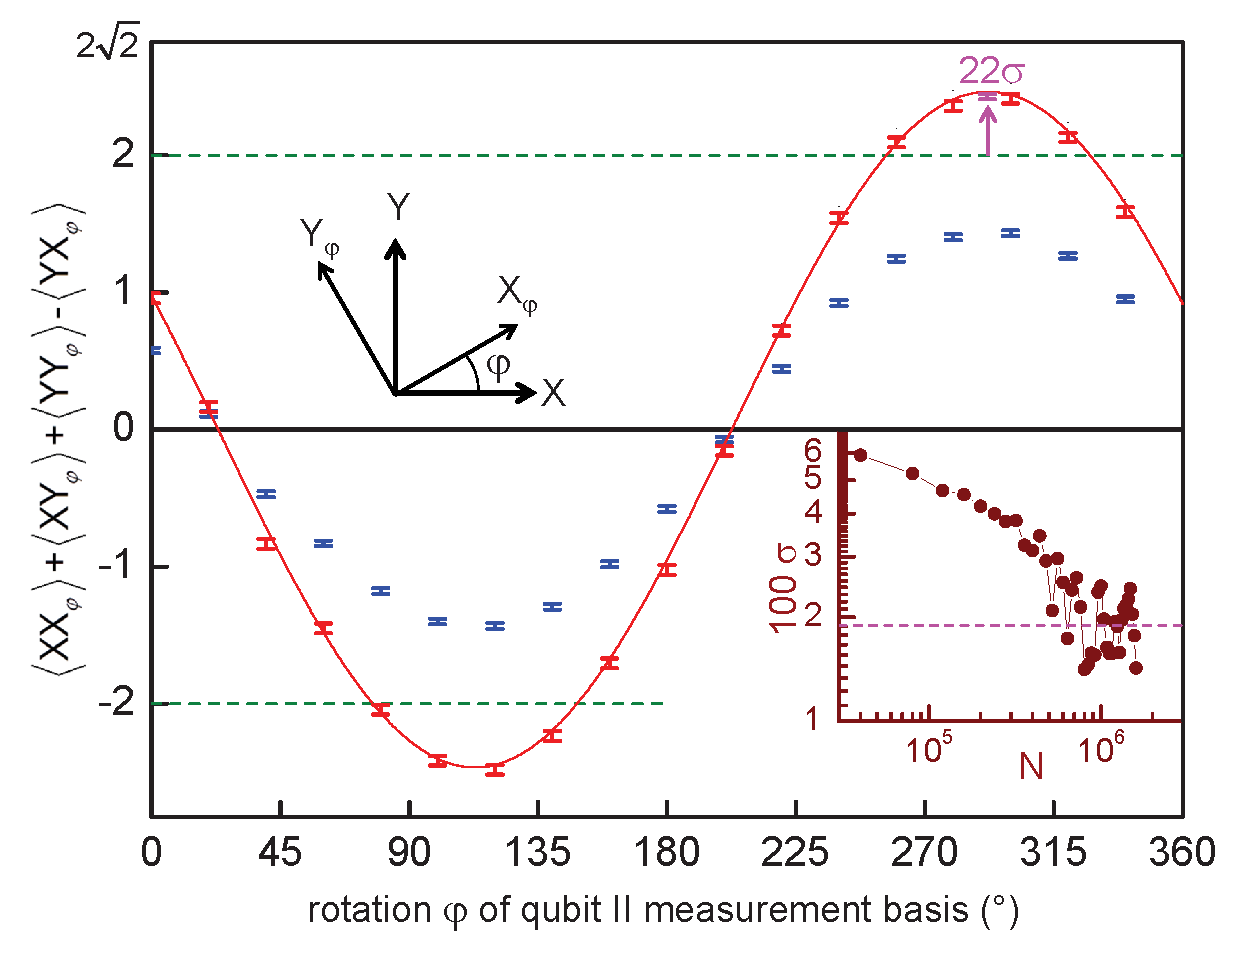
\includegraphics[width=0.7\textwidth]{./material/papers/iswap/submission1/Dewes_Figure3}
	\caption[Measurement of the CHSH operator of an entanged two-qubit state]{Measurement of the CHSH operator for an entangled two-qubit state. The renormalized CHSH expectation value (red points) exceeds the classical boundary of $2$ by a large amount. The raw measurement data (blue points) lies below this critical threshold. The inset shows the standard deviation $\sigma$ at the highest point of the curve as a function of the measurement sample size. For the highest sample count, the classical boundary is exceeded by $22$ standard deviations.\figcomment{p. 140 in cavities 6 labbook}}
	\label{fig:chsh_measurement}
\end{figure}

For classical states, the maximum value of the $\mathrm{CHSH}$ operator is bound by $2$ but for entangled states it can reach a maximum of $2\sqrt{2}$. Fig. \ref{fig:chsh_measurement} shows the result of such a $\mathrm{CHSH}$-type measurement performed on a state created by the method described above, showing the value of $\bracket{\mathrm{CHSH}}$ as a function of the angle $\phi$ of the measurement basis (more details about the measurement and the preparation of the entangled state can be found in the main text). We observe a violation of the classical boundary $2$ of the operator by $22$ standard deviations when correcting the readout errors that are present in our system. The raw, uncorrected data fails to exceed the non-classical bound due to readout errors mainly caused by qubit relaxation during the readout. Nevertheless, the observed violation of the equation in the renormalized measurement data is a strong indication of entanglement in the system.

\section{Realizing a Universal Two-Qubit Quantum Gate}

\begin{SCfigure}[][htb!]
		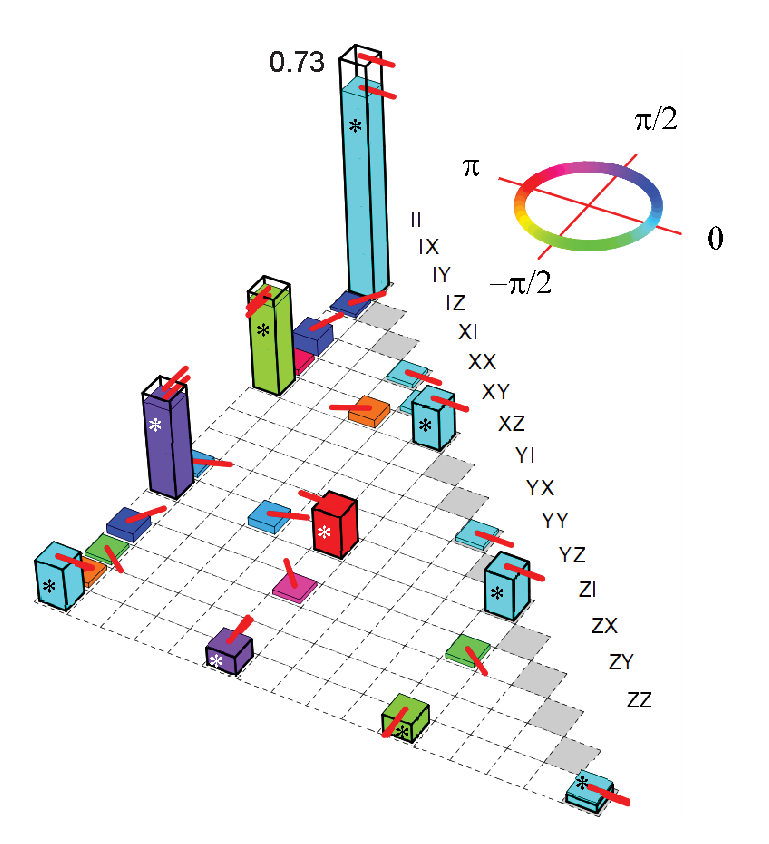
\includegraphics[width=0.65\textwidth]{./material/papers/iswap/figures/chi_matrix}
	\caption[Measured $\chi$-matrix of the $\sqrt{i\textrm{SWAP}}$ gate]{The measured $\chi$-matrix of the implemented $\sqrt{i\mathrm{SWAP}}$ gate. The row labels correspond to the indices of the $E_i$ operators, the height of each bar to the absolute value of the corresponding matrix element and the color and direction of the red arrow to the complex phase of each element. The ideal $\chi$-matrix of the $i\sqrt{\mathrm{SWAP}}$ gate is given by the outlined bars. The upper half of the positive-hermitian matrix is not shown.}
	\label{fig:gate_chi_matrix_and_errors}
\end{SCfigure}

The swapping evolution given by eq. (\ref{eq:swap_evolution_operator}) allows not only the preparation of entangled two-qubit states but also the implementation of a two-qubit gate. When switching on the interaction for a time $t_{\pi/2} = 1/8g$ we can realize the so-called $\sqrt{i\mathrm{SWAP}}$ gate, which has the representation

\begin{equation}
	U(t)  =  \left( \begin{array}{cccc} 1 & 0 & 0 & 0 \\ 0 & 1/\sqrt{2} & i\sqrt{2} & 0 \\ 0 & i\sqrt{2} & 1/\sqrt{2} & 0 \\ 0 & 0 & 0 & 1 \end{array} \right) \label{eq:sqrt_iswap_gate}
\end{equation}

and is a universal two-qubit quantum gate. We characterize the operation and errors of our implementation of this gate by performing quantum process tomography, obtaining a gate fidelity of 90 \%\ . The 10 \% error in gate fidelity is caused mainly by qubit relaxation and dephasing during the gate operation and only marginally by deterministic preparation errors, as will be discussed in the main text of the thesis. Fig. \ref{fig:gate_chi_matrix_and_errors} show the measured $\chi$ matrix of the gate, which contains the full information on the unitary and non-unitary action of the gate. The achieved fidelity of the gate operation is sufficient to allow the implementation of a simple quantum algorithm with our processor, as will be discussed in the following section.
 
\section{Running a Quantum Search Algorithm}

\begin{figure}[ht!]
	\centering
		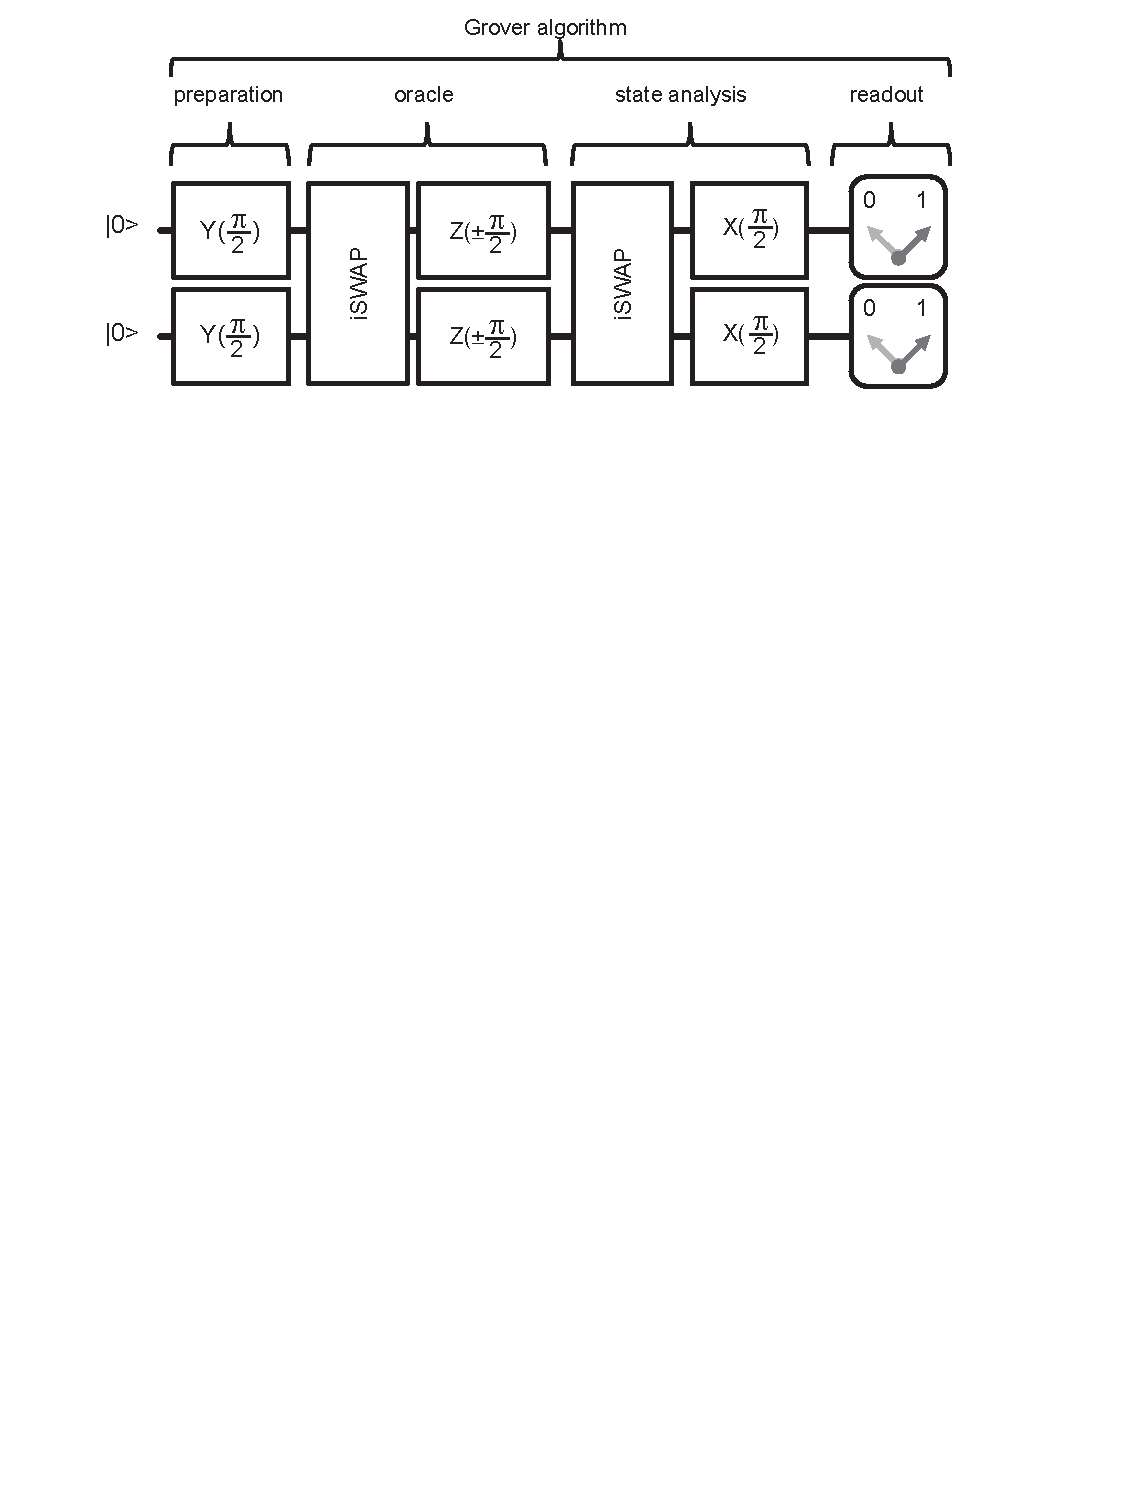
\includegraphics[width=0.8\textwidth]{./material/papers/grover/figures/grover_algorithm_schematic}
	\caption[Schematic of the implementation of the Grover search algorithm]{Schematic of the implementation of the Grover search algorithm on our two-qubit quantum processor. The algorithm consists in preparing a fully superposed state, applying the quantum Oracle operator to this state and analyzing the resulting output to determine the operator that has been applied with only a single call to the Oracle function.} 
	\label{fig:grover_algorithm_schematic}
\end{figure}

We can use a two-qubit quantum gate derived from the one described above to run a simple quantum algorithm on our processor, the so called {\it Grover search algorithm} \citep{Grover_Quantum_1997}. The version of this algorithm that we implemented operates on a two-qubit basis $x_i \in \{$ $\ket{00}$ , $\ket{01}$, $\ket{10}$ , $\ket{11}\}$ and can distinguish between four different {\it Oracle functions} $f(x)$ with $x \in x_i$ that each tag one given basis state $x_j$. In the two-qubit case, this algorithm requires only one evaluation of the Oracle function $f(x)$ to determine which state has been marked by the Oracle operator and is therefore faster than any classical algorithm, which would need at most three evaluations of the Oracle function to determine it with certainty. Therefore, it demonstrates the concept of quantum speed-up in a straightforward and intuitive way. The schematic of our version of the Grover algorithm is shown in fig. \ref{fig:grover_algorithm_schematic} and involves two $i\mathrm{SWAP}$ gate operations and six single-qubit operations along with a single-shot qubit readout at the end of the algorithm. We implemented this algorithm with our two-qubit processor and performed quantum state tomography after each step to reconstruct the quantum state at different points in the algorithm. 

\begin{figure}[ht!]
	\centering
		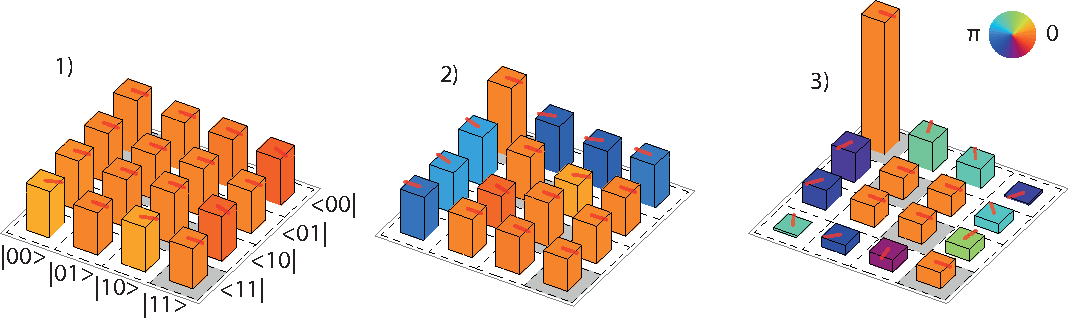
\includegraphics[width=1.\textwidth]{./material/figures/2-qubit-processor/grover/grover-density-matrices-state-1}
	\caption[Measured density matrices when running the Grover algorithm]{Measured density matrices when running the Grover search algorithm with a search oracle marking the state $\ket{00}$. 1) shows the state after the generalized Hadamard transform, 2) after applying the quantum oracle and 3) after the final step of the algorithm.} 
	\label{fig:grover_density_matrices_state_1}
\end{figure}

Fig. \ref{fig:grover_density_matrices_state_1} shows the experimentially measured density matrices when running this algorithm with an Oracle operator that marks the state $\ket{00}$. State tomographies are shown after applying a generalized Hadamard transform to the initial state $\ket{00}$, after evaluating the quantum Oracle function and after the final step of the algorithm. The measured state tomographies after the final state of the algorithm yield state fidelities of $68 \%$, $61 \%$, $64 \%$ and $65 \%$ for the four different Oracle functions, respectively. These fidelities have been corrected for readout errors and therefore do not quantify the quantum speed-up that can be achieved when running this algorithm with our processor. For this it is necessary to analyze the uncorrected single-shot readout outcomes, which we will do in the next section, showing that it is possible to demonstrate a form of probabilistic quantum speed-up with our processor.

\section{Demonstrating Quantum Speed-Up}

\begin{figure}[ht!]
		\centering
		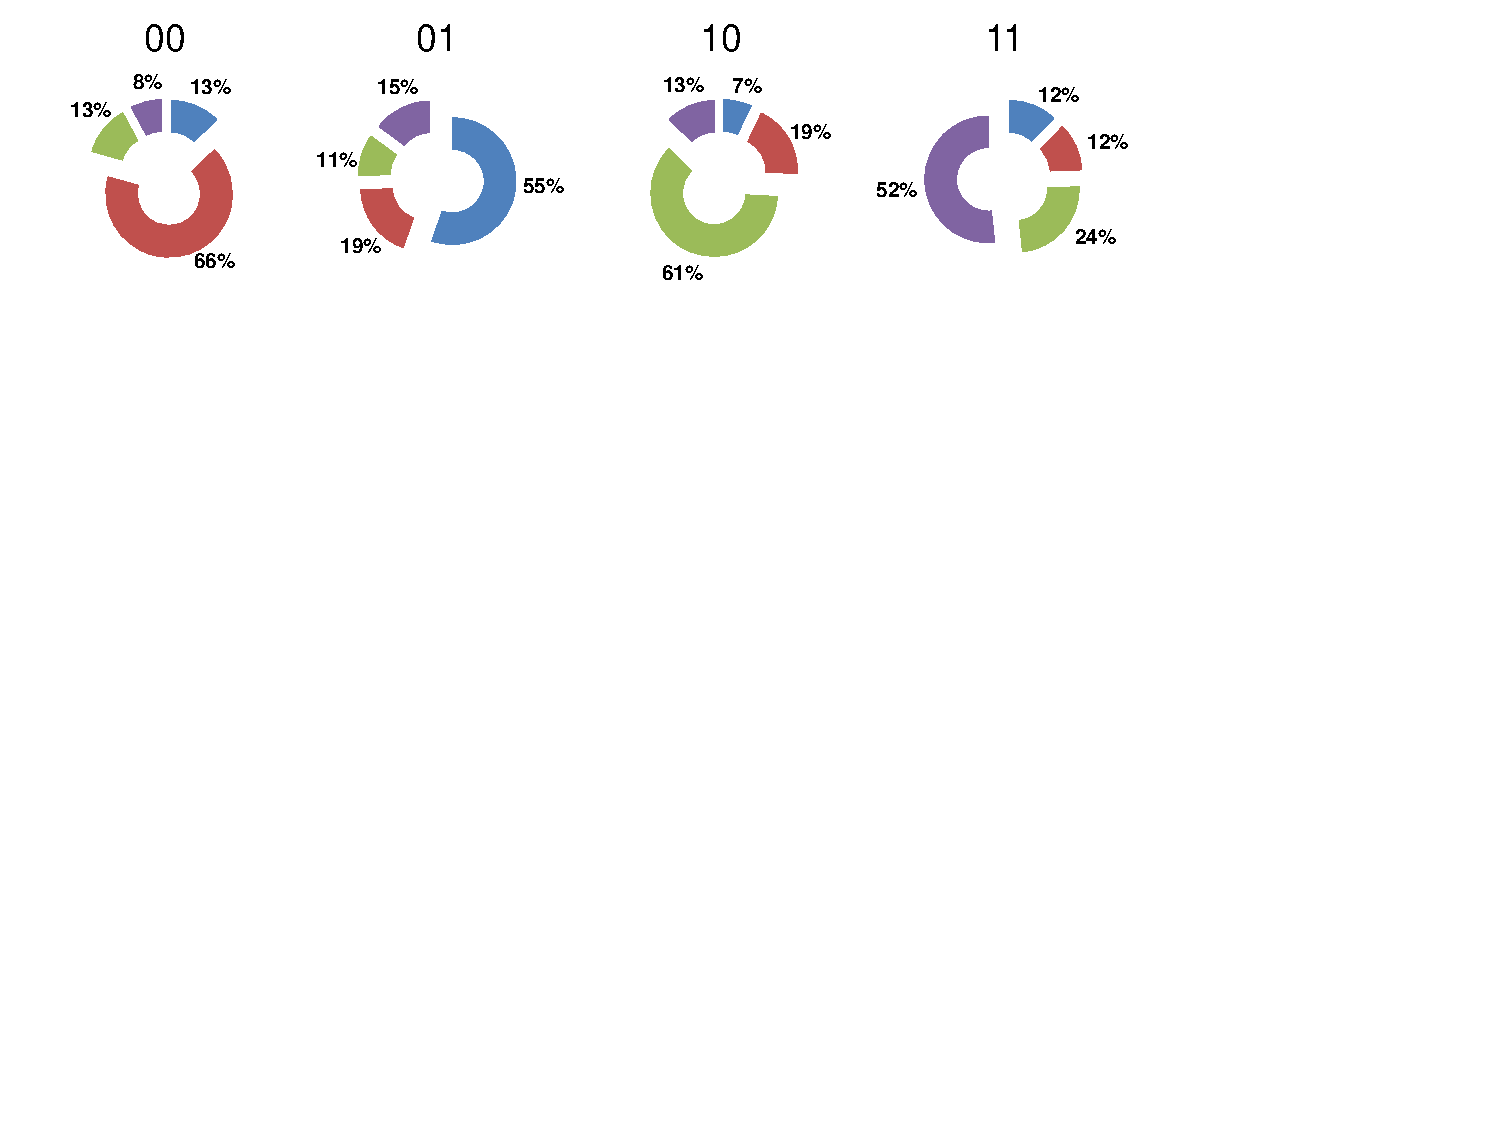
\includegraphics[width=1.0\textwidth]{./material/papers/grover/figures/grover_algorithm_single_shot_probabilities}
	\caption[Single-run results of the Grover search algorithm]{Single-run results when running the Grover search algorithm on our two-qubit quantum processor. Shown are the probabilities of obtaining the results $00,01,10,11$ as a function of the Oracle function provided to the algorithm, indicated by the number on top of each graph. In all four cases, the success probability of the algorithm is $> 50 \%$, thus outperforming any classical query-and-guess algorithm in the required number of calls to the Oracle function.}
	\label{fig:grover_single_shot_probabilities}
\end{figure}

The main interest of running a quantum algorithm is to obtain an advantage in the run-time in comparision to a classical algorithm, the so-called {\it quantum speed-up}. To characterize this quantum speed-up as obtained with our processor, we run the Grover algorithm for all four possible Oracle functions and directly read out the state of the qubit register after the last step of the algorithm instead of performing quantum state tomography, thus not correcting any readout errors. By averaging the outcomes of many such individual runs of the algorithm with different Oracle functions we obtain the so-called {\it single-run fidelities}, which --for the four different Oracle functions-- have been measured as $66 \%$, $55\%$, $61\%$ and $52\%$. The full probability distributions for the four possible cases and are shown in fig. \ref{fig:grover_single_shot_probabilities}. The measured success probabilities that are $> 50 \%$ demonstrate the probabilistic quantum speed-up achieved with our processor compared to a classical query-and-guess algorithm that would be able to give the correct answer with only $50\%$ single-run fidelity (a detailed explanation of this value can be found in the section on the Grover search algorithm in the main part of this thesis). The achieved success probabilities still are considerably lower than the theoretically possible values of 100 \% , where the errors are mainly due to relaxation and decoherence of the qubit state during the runtime of the algorithm and to a small degree also due to errors in the pulse sequence.